%%%%%%%%%%%%%%%%%%%%%%% file template.tex %%%%%%%%%%%%%%%%%%%%%%%%%
%
% This is a general template file for the LaTeX package SVJour3
% for Springer journals.          Springer Heidelberg 2010/09/16
%
% Copy it to a new file with a new name and use it as the basis
% for your article. Delete % signs as needed.
%
% This template includes a few options for different layouts and
% content for various journals. Please consult a previous issue of
% your journal as needed.
%
%%%%%%%%%%%%%%%%%%%%%%%%%%%%%%%%%%%%%%%%%%%%%%%%%%%%%%%%%%%%%%%%%%%
%
% First comes an example EPS file -- just ignore it and
% proceed on the \documentclass line
% your LaTeX will extract the file if required
%
\RequirePackage{fix-cm}
%
%\documentclass{svjour3}                     % onecolumn (standard format)
%\documentclass[smallcondensed]{svjour3}     % onecolumn (ditto)
\documentclass[smallextended]{svjour3}       % onecolumn (second format)
%\documentclass[twocolumn]{svjour3}          % twocolumn
%
\smartqed  % flush right qed marks, e.g. at end of proof
%
%----------------------------------------
\usepackage{graphicx}
\usepackage{amsmath}
\usepackage{amssymb, stmaryrd}
\usepackage{subfig}
\usepackage{caption}
\usepackage{cite}
\usepackage{enumitem}
\usepackage{filecontents}
\usepackage{listings}
\usepackage{mathtools, cuted}
\usepackage{tikz}
\usepackage{algorithm}
\usepackage{algpseudocode}
\usepackage[textwidth=17mm]{todonotes}
\usetikzlibrary{calc,arrows,shapes,automata,petri,positioning,decorations.markings,shadows}
\usepackage{subfig}

\tikzset{
    use/.style={
    circle,draw=black,fill=black,scale=0.5,text=white
    },
    mpi/.style={
    rectangle,draw=black,fill=black,scale=0.8,text=white
    },
    provide/.style={
    circle,draw=black,fill=white,scale=0.5
    },
    component/.style={
    rectangle,rounded corners=3pt,draw=black
    },
    dcomponent/.style={
    rectangle,rounded corners=3pt,dashed,draw=black
    },
}

\usepackage{url}
\usepackage{xspace}
\usepackage{color}

% comments
\newcommand{\customtodo}[4]{
        \todo[color=#2,inline,size=\small]{
                \ifx&#3&
                        \textbf{#1} #4
                \else
                        \textbf{#1$\Rightarrow$#3} #4
                \fi
        }
}
\newcommand{\HC}[2][]{\customtodo{HC}{red!20}{#1}{#2}}
\newcommand{\CP}[2][]{\customtodo{CP}{blue!20}{#1}{#2}}
\newcommand{\JB}[2][]{\customtodo{JB}{green!20}{#1}{#2}}

\newcommand{\ie}{\emph{i.e.,}\xspace}
\newcommand{\eg}{\emph{e.g.,}\xspace}
\newcommand{\llc}{L\textsuperscript{2}C\xspace}

%\newtheorem{theorem}{Theorem}[section]
\newtheorem{myprop}[theorem]{Proposition}
\newtheorem{mydef}[theorem]{Definition}
\newtheorem{myth}[theorem]{Theorem}
\newenvironment{mydefs}[1][Definitions]{\par\medskip\noindent\textbf{#1}\nopagebreak\begin{itemize}[noitemsep,topsep=.25\topsep]}{\end{itemize}}

\def\pprec{\mathrel{\scalebox{.9}[1]{$\prec$}\mkern-3mu%
  \scalebox{.4}[1]{$\prec$}\mkern-5.5mu\scalebox{.4}[1]{$\prec$}}}
%----------------------------------------
 
%----------------------------------------
\begin{document}
%----------------------------------------

%----------------------------------------
\title{The Multi-Stencil Framework: A Component-Based Approach to Orchestrate Stencils}
%----------------------------------------
\author{H\'el\`ene Coullon \and Julien Bigot \and Christian Perez}
%----------------------------------------
\institute{H\'el\`ene Coullon \at
              DAPI IMT Atlantique, LS2N, Inria. Nantes, France\\
              \email{helene.coullon@inria.fr}
	\and
           Julien Bigot \at
           Maison de la Simulation, CEA, CNRS, Univ. Paris-Sud, UVSQ, Universit\'e Paris-Saclay, 91191 Gif-sur-Yvette, France\\
           \email{julien.bigot@cea.fr}           
           \and
	Christian Perez \at
              Univ. Lyon, Inria, CNRS, ENS de Lyon. Lyon, France\\
              \email{christian.perez@inria.fr}
}
%----------------------------------------
\maketitle
%----------------------------------------
\begin{abstract}
As the computation power of modern high performance architectures increases, their heterogeneity and complexity also become more important. One of the big challenges of exascale is to reach programming models that give access to high performance computing (HPC) to many scientists and not only to a few HPC specialists. One relevant solution to ease parallel programming for scientists is Domain Specific Language (DSL). However, one problem to avoid with DSLs is to mutualize existing codes and libraries instead of implemented each solution from scratch. For example, this phenomenon occurs for stencil-based numerical simulations, for which a large number of languages has been proposed without code reuse between them. 
The Multi-Stencil Framework (MSF) presented in this paper combines a new DSL to component-based programming models to enhance code reuse and separation of concerns in the specific case of stencils. MSF can easily choose one parallelization technique or another, one optimization or another, as well as one back-end implementation or another. It is shown that MSF can reach same performances than a non component-based MPI implementation over 16.384 cores. Finally, the performance model of the framework for hybrid parallelization is validated by evaluations.

\keywords{Component programming models \and Domain Specific Language (DSL) \and Stencil \and Numerical simulation \and Data parallelism \and Task parallelism \and Scheduling \and MPI \and OpenMP}
\end{abstract}
%------------------------------------------------------------------------------
\section{Introduction}
\label{sect:introduction}
As the computation power of modern high performance architectures increases, their heterogeneity and complexity also become more important. For example, the current world's top supercomputer Tianhe-2~\footnote{url{www.top500.org}} is composed of multi-cores processors and accelerators, and is able to reach a theoretical peak performance around thirty floating point operations par seconds. However, to be able to use such a machine, multiple programming models, such as MPI (Message Passing Interface), OpenMP, CUDA etc., and multiple optimization techniques, such as cache optimizations or vectorization optimizations, have to be combined. Moreover, current architectures evolution lets think that heterogeneity and complexity in HPC will continue to grow in future.

One the big challenges to solve to be able to use exascale computers is to propose programming models which gives access to high performance computing (HPC) to many scientists and not only to a few HPC specialists~\cite{ETP4HPC2013}. Actually, applications which run on supercomputers and which need such a computation power are physics, weather or genomic applications, which are not implemented by HPC specialists most of the time.

Many low level execution models focuss onto the dynamic scheduling of task graphs combined to message passing models to be able to use more than one machine~\cite{Gautier:2013:XRS:2510661.2511383,Augonnet2011,wu:hal-01078359}. Those models increase HPC code portability and reach an interesting performance onto heterogeneous architectures, which is interesting to reach exascale programming. At a higher abstraction level, general purpose parallel languages, such as OpenMP~\cite{660313} and OpenCL~\cite{Stone:2010:OPP:622179.1803953} follow the direction of task graph scheduling proposed by those execution models. However, for non-experts end-users, general purpose languages still are difficult to use and to tune for a given application onto a given architecture. The current easiest (with the higher abstraction level), but still efficient, programming model for end-users is Domain Specific Language (DSL). Such a language is specific to the end-user domain and proposes a grammar which is easy to understand. The DSL compiler is able, because of the specific knowledge onto the domain targetted, to automatically apply parallelization and specific optimizations to produce a high performance back-end code. Thus, a DSL is able to split end-user concerns from HPC concerns which is relevant to reach exascale programming models.

However, many DSLs have been proposed for many domains yet, and, as far as we know, only a few of them have been able to reuse work already done by another language~\cite{Sujeeth:2013:CRC:2524984.2524988}. In other words, software engineering properties have to be integrated into DSL conception, such that a new DSL can be seen as a composition of parallelization, optimizations or even languages semantics already proposed by others.

For example, to numerically solve a set of partial differential equations (PDEs), iterative methods are frequently used to approximate the exact solution through a discretized phenomena. A very well known and usual way to discretize PDEs is to transform them to explicit numerical schemes, also often called \emph{stencils}. Many DSLs have been proposed for stencil computations~\cite{spaaTangCKLL11,citeulike12258902,Ragan-Kelley:2013:HLC:2491956.2462176,DeVito:2011:LDS:2063384.2063396,Camier:2015:IPP:2820083.2820107}, as it will be detailed in Section~\ref{sect:rel}. Many of them use same kind of parallelization, data structures or optimizations, however each one has been built from scratch to deal with another additionnal specific case.
We present the Multi-Stencil Language (MSL) DSL, also for stencil-based numerical simulations. MSL is a language with a light grammar to describe a numerical simulation without implementation details. From the description, the compiler has enough information to extract and build an empty parallel pattern of the simulation, which can be filled, in a second step, by implementation concerns. The parallel pattern generated by the language is able to use different existing languages and libraries as it is independent from implementation choices. Moreover, the parallelization performed by the language is large enough to be compatible with many architectures and back-end languages. Contributions presented in this paper are : the computational model of a multi-stencil program and its parallelization formalism; the MSL grammar and its compiler; and a performance evaluation of a real case numerical simulation up to 16.384 cores.

Section~\ref{sect:rel} introduces related work on stencils DSLs. Section~\ref{sect:formalism} formally explains the targetted domain and its computational model. From this model can be extracted the grammar of MSL in Section~\ref{sect:msl}. Section~\ref{sect:parallelism} shows how parallelism can be extracted from this light grammar of MSL. Sections~\ref{sect:msp} and~\ref{sect:comp} detail choices that have been done in this paper to evaluate MSL, and Section~\ref{sect:eval} shows performance results of the language. Finally, Section~\ref{sect:concl} concludes and proposes perspectives on this work.
%------------------------------------------------------------------------------
\section{The Component-Based Multi-Stencil Framework}
\label{sect:msf}
\HC{under construction, present the framework}

This section first presents a background on component models and particularly on the Low Level Components. This background is needed to understand the second part of the section which presents an overview of the overall Multi-Stencil Framework (MSF).

%----------------------------------------
\subsection{Background on component models}
%----------------------------------------
Component-based software engineering (CBSE) is a domain of software engineering~\cite{Szyperski:2002:CSB:515228} which improves code re-use, separations of concerns, and thus maintainability.
An component-based application is made of a set of component instances linked together, this is also called a component \emph{assembly}.
A component is a black box that implements an independent functionality of the application, and which interacts with its environment only through well defined interfaces: its ports.
A port can, for example, specify services provided or required by the component.
With respect to high performance computing, some works have also shown
that component models can achieve the needed level of performance, and
scalability while also helping in application portability~\cite{Bernholdt01052006, bigot:inria-00388508, UCHPC2015}

Many component models exist, each of them with its own specificities.
Well known component models include, for example, the CORBA Component Model (CCM)~\cite{corba:omg06}, and the Grid Component Model (GCM)~\cite{Baude} for distributed computing, while the Common Component Architecture (CCA)~\cite{Bernholdt01052006}, and Low Level Components (\llc)~\cite{l2c} are HPC-oriented.
This work makes use of \llc for the experiments.

\llc~\cite{l2c} is a minimalist \texttt{C++} based HPC-oriented component model
where a component extends the concept of class.
The services offered by the components are specified trough $provide$ ports,
those used either by $use$ ports for a single service instance,
or $use-multiple$ ports for multiple services instances.
Services are specified as \texttt{C++} interfaces.
\llc also offers $MPI$ ports that enable components to share MPI communicators. Finally, 
components can also have attribute ports to be configured.
%
In this paper, and as illustrated in Figures~\ref{fig:ports}, a $provide$ port is represented by a white circle, a $use$ port with a black circle, a $use-multiple$ port by a black circle with a white $m$ in it. MPI port are connected with a black rectangle. A \llc-based application is a static \emph{assembly} of components instances and the connections between their ports.
Such an assembly is described in LAD, an XML dialect.

\begin{figure}[t]
\begin{center}
\subfloat[][\label{fig:2comp}]{
\begin{tikzpicture}[shorten >=1pt, node distance=2cm, on grid, auto]
   \node[component] (C) at (0,0) {$c_0$};
   \node[provide] (p) at (-1.5,0) {};
   \node[use] (u) at (1.5,0) {};
   \node[provide,right=1.5cm of u] (p1) {};
   \node[component,right=1.5cm of p1] (C1) {$c_1$};
   \node[use,right=1.5cm of C1] (um) {$m$};
 
  \path[-]
    (p) edge node {$p$} (C)
    (C.east) edge node {$u$} (u)
    (C1)  edge node {$v$} (um)
    (p1) edge node {$q$} (C1);
\end{tikzpicture}
}
\\
\subfloat[][\label{fig:ass}]{
\begin{tikzpicture}[shorten >=1pt, node distance=2cm, on grid, auto]
   \node[component] (C) at (0,0) {$c_0$};
   \node[provide] (p) at (-1.5,0) {};
   \node[use] (u) at (1.5,0) {};
   \node[provide,right=0.15 of u] (p2) {};
   \node[component,right=1.5 of p2] (C1) {$c_1$};
   \node[use,right=1.5 of C1] (um) {$m$};
 
  \path[-]
    (p) edge node {$p$} (C)
    (C) edge node {$u$} (u)
    (C1)  edge node {$v$} (um)
    (p2) edge node {$q$} (C1);
\end{tikzpicture}
}
\\
\subfloat[][\label{fig:mpi}]{
\begin{tikzpicture}[shorten >=1pt, node distance=2cm, on grid, auto]
   \node[component] (C) at (0,0) {$c_2$};
   \node[provide] (p) at (-1.5,0) {};
   \node[mpi] (u) at (1.5,0) {};
   \node[component,right=1.5 of u] (C1) {$c_3$};
 
  \path[-]
    (p) edge node {} (C)
    (C) edge node {} (u)
    (u) edge node {} (C1);
\end{tikzpicture}
}
\caption{Example of components and their ports representation. a) Component $c_0$ has a provide port ($p$) and a use port ($u$); Component $c_1$ has also a provide port ($q$) but also a use multiple port ($v$). b) A use port is connected to a (compatible) provide port. c) Component $c_2$ and $c_3$ shares an MPI communicator.}
\label{fig:ports}
\end{center}
\end{figure}

%----------------------------------------
\subsection{Multi-Stencil Framework overview}
%----------------------------------------
The Multi-Stencil Framework helps end-users to produce high performance parallel applications for the specific case of multi-stencils. The multi-stencil domain will be formally defined in the next section. A multi-stencil program is typically a numerical simulation based on explicit numerical schemes that approximate PDEs equations with one or multiple neighborhood computations.

Figure~\ref{fig:msf} presents the overview of the Multi-Stencil Framework that will be entirely detailed throughout this paper. It is composed of four different parts presented below.

One can note in this figure that MSF is addressed to two different kinds of end-users: the \emph{numerician}, in other words the mathematician, and the \emph{developer}. Most of the time numericians do have programming knowledge, however as it is not their core domain and because of a lack of time, development is often left to engineers according to numericians needs. MSF has the interesting particularity to propose a clear separation of concerns between these two end-users by distinguishing the description language from the numerical code. 

MSF also has the interesting capability to become flexible thanks to a third user possibility to interact with the framework: the High Performance Computing (HPC) specialist.

\begin{figure}[t]
\begin{center}
  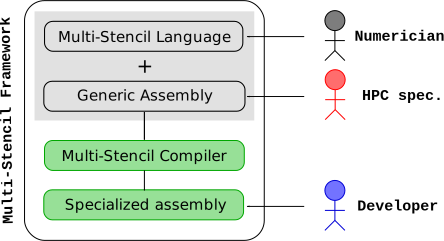
\includegraphics[width=.6\textwidth]{./images/msf.pdf}
  \caption{The Multi-Stencil Framework (MSF) composed of the Multi-Stencil Language (MSL), the Generic Assembly (GA), the Multi-Stencil Compiler (MSC) and which produces a specialized assembly of components.}
  \label{fig:msf}
\end{center}
\end{figure}

\paragraph{\textbf{Multi-Stencil Language}}
The Multi-Stencil Language, or MSL, is the domain specific language proposed by the framework for the numerician. It is a descriptive language, easy to use, without any concern onto implementation details, which fits the need of a mathematician to describe the simulation. The description written with MSL can be considered as an input of the framework. MSL is described in details in Section~\ref{sect:msl}. The language is built upon the meta-model described in Section~\ref{sect:formalism}.

\paragraph{\textbf{Generic Assembly}}
In addition to the language MSL and the simulation description written by the numerician, MSF needs a generic assembly of a multi-stencil program as input. What is called a generic assembly is a component assembly for which meta-types are represented and for which some parts need to be generated or specialized. It is similar to a generic pattern or a skeleton in usual programming models such as C++ or functional models. From this generic assembly will be built the final specialized assembly of the simulation. As well as MSL, this generic assembly is described in Section~\ref{sect:msl} and is built upon the meta-model described in Section~\ref{sect:formalism}. Moreover, an example of generic assembly is used in evaluations of Section~\ref{sect:eval}.
\HC{Note idée : HPC specialist gives types for DDS and Data}

\paragraph{\textbf{Multi-Stencil Compiler}}
The core of the framework is the Multi-Stencil Compiler, or MSC. It is responsible for transforming the genric assembly into the final parallel assembly which is specific to the simulation described by the numerician. MSC is described in Sections~\ref{sect:parallelism} and~\ref{sect:msp}.

\paragraph{\textbf{Specialized assembly}}
Finally, the input of MSF is the component assembly generated by MSC. It is an instanciation and a transformation of the generic component assembly, by adding component types and by adding specific components generated by MSC. From this final component assembly which is specific to the simulation initially described by using MSL, the developer will finally write numerical codes.
%------------------------------------------------------------------------------
\section{Formalism of a Multi-Stencil Program}
\label{sect:formalism}
To numerically solve a set of PDEs, iterative methods (finite difference, finite volume or finite element methods) are frequently used to approximate the solution through a discretized (step by step) phenomena. Thus, the continuous time and space domains are discretized so that a set of numerical computations are iteratively (time discretization) applied onto a mesh (space discretization). In other words, the PDEs are transformed to a set of numerical computations applied at each time step on all elements of the discretized space domain. Among those numerical computations is found a set of numerical schemes, also called \textit{stencil computations}, and a set of auxiliary computations also needed to perform the simulation, and also called \emph{local computations}.
This section gives formal definitions of a \textit{stencil program} and its computations. Then, the different parallelization techniques which can be applied on such program, are presented.

%-------------------------------------
\subsection{Time, mesh and data}

A mesh $\mathcal{M}$ defines the discretization of the continuous space domain $\Omega$ of a set of PDEs and is defined as followed. 

\begin{mydef}
\textit{A mesh is a connected undirected graph $\mathcal{M}=(V,E)$, where $V$ is the set of vertices and $E$ the set of edges. The set of edges $E$ of a mesh $\mathcal{M}=(V,E)$ does not contain bridges.}
\end{mydef}

\rmq{Pas très clair la suite; motivation? dom == some sub elements of M ?}
\begin{mydef}
$D_i$ is a set of elements of a mesh $\mathcal{M}=(V,E)$, constructed by a function $dom_i$ which defines a precise association between $V$ and $E$, $dom_i : V \times E \rightarrow D_i$.
\end{mydef}
For example, the set of cells $D_0$ in a Cartesian 2D mesh could be defined by exactly four vertices and four edges connected as a cycle. But we could also define another set of elements $D_1$ as the simple set of vertices $V$, etc.

A mesh can be structured (as Cartesian or curvilinear meshes), unstructured, regular or irregular (without the same topology for each element) and hybrid. 

\begin{figure}[!h]\begin{center}
  \resizebox{8cm}{!}{\includegraphics{./images/maillages.pdf}}
  \caption{From left to right, Cartesian, curvilinear and unstructured meshes.}
  \label{fig:mesh}
\end{center}\end{figure}

\begin{mydef}
The discretization of the continuous time domain $\mathcal{T}$ is denoted $T$ such that $\forall\mbox{ }t_i\mbox{, }t_{i+1} \in T\mbox{, }\exists\mbox{ }\Delta t \in \mathbb{R}$\mbox{, }$t_{i+1} = t_i + \Delta t$. Thus, $T$ is responsible for the iteration time steps of the numerical simulation. 
\end{mydef}

In a numerical simulation a set of data, or quantities, are applied onto the mesh and represent the set of values to compute, or to use, for computation.

\begin{mydef}
The set of data applied on the mesh is denoted by $\Delta$, such that $\delta \in \Delta$ is a function which associates each element $d \in D_i$ (the domain it is applied on) to a value $v \in V$, $\delta : D_i \rightarrow V$. In the rest of this paper, the domain of a data $\delta$ can be given by the function $domain(\delta)=D_i$.
\end{mydef}
One can notice that in applied mathematics, the signature of $\delta$ would be $\delta : D_i \times T \rightarrow V$, however when programming a numerical simulation it is not wise to store all values of each time iteration.

%-----------------------
\subsection{Computations}

\begin{mydef}
A numerical expression $\text{exp}$ is a function which represents how to compute a value for an element $d \in domain(w)=D_i$, using the set $R \subset \Delta$ of input data (read data), $\text{exp} : R \times D_i \rightarrow w \times D_i$.
\end{mydef}

\begin{mydef}
A computation $c$ of a numerical simulation is defined as $c(R,w,\text{exp})$, where $R \subset \Delta, w \in \Delta$ and $\text{exp}$ a numerical expression. %$D$ is one of the subsets $D_i \subset \mathcal{M}$, such that $w : D \rightarrow V$.
\end{mydef}
It has to be noticed that at each time iteration, all the elements of a mesh are computed. However, it happens that computations of the mesh elements are splitted in different domains, as for example the computation of the physical border. In this case additional $D_i$ can be specified for the mesh $\mathcal{M}$.

\begin{mydef}
The set of $n$ ordered computations of a numerical simulation is denoted $\Gamma = [c_i]_{0 \leq i \leq n-1}$, such that $\forall c_i,c_j \in \Gamma$, if $i \leq j$, then $c_i$ is computed before $c_j$, and $c_j$ can be computed only when $c_i$ is finished.
\end{mydef}

\begin{mydef}
A \textit{multi-stencil program} is defined by the quadruplet $\mathcal{MSP}(T,\mathcal{M},\Delta,\Gamma)$.
\end{mydef}
%If the number of computations in $\Gamma$ is $card(\Gamma)=n$, such that $\bigcup_{i=0}^{n-1}c_i = \Gamma$, then $\bigcup_{i=0}^{m-1}R_i \cup w_i \subseteq \Delta$.

As already mentioned, the ordered list $\Gamma$ can be composed of two different types of computations, stencil and local computations, which will be defined in the rest of this Section.

\begin{mydef}
The neighborhood $\mathcal{N}$ of an element $d \in D_i$ is a function to obtain a set of elements in any $D_k \subset \mathcal{M}$, $\mathcal{N} : D_i \rightarrow D_k \times D_k \times \dots$.
\end{mydef}
The function $\mathcal{N}$ is also sometimes called the \textit{stencil shape}, or the \textit{stencil} in applied mathematics. In this paper we distinguish a stencil shape from a \textit{stencil computation} defined as followed:

\begin{mydef}
A \textit{stencil computation} is defined as a quadruplet $s(R,w,\text{exp},\mathcal{N})$, where $R \subset \Delta$, and $w : D \rightarrow V \in \Delta$.
\end{mydef}
In a stencil computation $s$, $\forall d \in D$, the stencil numerical expression $\text{exp}$ is applied such that $w(d) = \text{exp}(R(d),R(\mathcal{N}(d))$. In this work, a stencil computation $s(R,w,\text{exp},\mathcal{N})$ always verifies $R \cap \{w\} = \emptyset$, otherwize an implicit numerical scheme has to be solve which is over the scope of this paper. As a result, the ordered list $\Gamma$ of a multi-stencil program can be composed of a set of stencil computations applied on one or more stencil shapes.

Figure~\ref{fig:ex} gives an example of a stencil computation $s(R,w,\text{exp},\mathcal{N})$, where $\mathcal{M}(V,E)$ is a two dimensional Cartesian mesh. A single domain $D=domain(w)$ is defined in this example and is composed of cells formed by a cycle of four vertices $v \in V$ and four edges $e \in E$. Furthermore, in this example $R=\{A\}$, $w=B$, and for $(x,y) \in D$ the neighborhood function is 
\begin{equation*}
\mathcal{N} : (x,y) \rightarrow \{(x,y+1),(x,y-1),(x+1,y),(x-1,y)\}.
\end{equation*}
Finally, the numerical expression of this example is 
\begin{equation*}
\text{exp}(A(x,y),A(\mathcal{N}(x,y)) = B(x,y) = A(x,y)+(A(x,y+1)+A(x,y-1)+A(x+1,y)+A(x-1,y))/4.
\end{equation*}

\begin{figure}[!h]\begin{center}
  \resizebox{8cm}{!}{\includegraphics{./images/example.pdf}}
  \caption{Example of a stencil computation.}
  \label{fig:ex}
\end{center}\end{figure}

The second type of numerical computation is a local computation.
\begin{mydef}
A local computation is a triplet $l(R,w,\text{exp})$, where $exp$ does not involve a neighborhood function $\mathcal{N}$.
\end{mydef}

A stencil program and stencil and local computations have been formally defined in this section. This formalism is used in the next Section to define two parallelization techniques of a multi-stencil program.



%------------------------------------------------------------------------------
\section{Generic Asssembly and The Multi-Stencil Language}
\label{sect:msl}
From the fomalism detailed in the previous section, the Multi-Stencil Language and its grammar can already be given. The reason why this grammar is sufficient to automatically extract parallelism will be explained in the next section.

\medskip
The grammar of the Multi-Stencil Language is given in Figure~\ref{fig:grammar}. A Multi-Stencil program is composed of eight parts. 

\begin{enumerate}
\item The first part represents the mesh of the simulation $\mathcal{M}$. As a single mesh is for now supported by the language, and as the topology of the mesh is not needed by the language compiler, \textit{meshid} (line 1) is a terminal symbol of the grammar. 
\item The second part (line 2) represents the set of groups of mesh entities needed by the simulation $\Phi$. It is defined as a list of groups $\mathcal{G}$. Again, as mesh entities are defined using the topology of the mesh, a group of mesh entities \textit{group} (defined line 13) is a terminal symbol of the grammar.
\item The third part (lines 3 and 4) represents the set of computation domains of the simulation $\mathcal{D}$. It is defined as a list of domains, each one defined (lines 14 and 15) as a subpart of a group of mesh entities, using the symbol "in".
\item The fourth part (lines 5 and 6) of the program is linked to the third one. It offers a way to declare that two computation domains are independants (lines 16 and 17). Two given computation domains $D_1$ and $D_2$ are independants if and only if $D_1 \cap D_2 = \emptyset$. It uses the symbol "and" to describe that $D_1$ and $D_2$ are independants.
\item The fith part (lines 7 and 8) represents the set of stencil shapes used by the simulation $\mathcal{N}$. A stencil shape (lines 18 and 19) is defined as a function "from" a group of mesh entities "to" another group of mesh entities.
\item The sixth part (line 9) represents the set of quantities of the simulation $\Delta$. It is composed of a list of quantities (lines 20 and 21) for which each line (line 22) begins with a group of mesh entities and a list of \textit{quanityid} which are applied onto the given group.
\item The seventh part (line 10) represents the set of scalars of the simulation $\mathcal{S}$. Each scalar (line 23) is a terminal symbol.
\item Finally, the eith part (line 11) represents the simulation computations. It is composed of a list of loop (line 24). Each \textit{loop} (line 25) is composed of a \textit{time} loop composed of \textit{iteration} (which represents $T$), and of a set of \textit{computations} (which represents $\Gamma$).
\begin{itemize}
\item A time loop, denoted \textit{iteration} in the grammar, can be a numerical constant value, \textit{num}, which directly indicates the number of time iterations, or a convergence \textit{criteria}. The \textit{criteria} symbol represents the function $conv:\mathcal{S}^n \rightarrow bool$ of the formalism. To define a criteria the terminal \textit{criteriaid} has to be set, and between bracket are indicated a list of scalars to read.
\item Each computation of the list of \textit{computations} follows the information of the formalism $k(S,R,(w,D),comp)$ except the $comp$ function which is an implementation concern. To be more easy to write the syntax is different though.
\end{itemize}
\end{enumerate}

\begin{filecontents*}{grammar.txt}
program ::= "mesh:" meshid 
            "mesh entities:" listgroup
            "computation domains:" 
                      listcompdom
            "independent:"
                      listinde
            "stencil shapes:"
                      liststencil
            "quantities:" listquantities
            "scalar" listscalar
            listloop

listgroup ::= group listgroup |  group
listcompdom ::= compdom listcompdom |  compdom
compdom ::= compdomid "in" group
listinde ::= inde listinde |  inde
inde ::= compdomid "and" compdomid
liststencil ::= stencil liststencil | stencil
stencil ::= stencilid "from" group "to" group
listquantities ::= data listquantities |  quantity
quantity ::= group listquantityid
listquantityid ::= quantityid listquantityid |  quantityid
listscalar ::= scalar listscalar | scalar
listloop ::= loop listloop | loop
loop ::=  "time:" iteration
          "computations:" listcomp
iteration ::= num | criteria
criteria ::= criteriaid "(" listscalarread ")"
listscalarread ::= scalar listscalarread |  scalar
listcomp ::= comp listcomp |  comp
comp ::= dataid "[" compdomid "]=" compid "({"listscalarread
                                          "},{"listdataread "})"
listdataread ::= dataread listdataread |  dataread
dataread ::= dataid "[" stencil "]" |  dataid
\end{filecontents*}

\begin{figure}[!h]
  \hspace{5mm}
  \begin{minipage}[!h]{0.98\textwidth}
    {\lstinputlisting[basicstyle=\small,mathescape,frame=single,language=Python,numbers=left]{grammar.txt}}   
    \caption{Grammar of the Multi-Stencil Language. \label{fig:grammar}}
  \end{minipage}
\end{figure}

\paragraph{\textbf{Example}} To give a better idea of a multi-stencil program, a short example is given in Figure~\ref{fig:exmsl}. In this example, the mesh is called \textit{cart}. Two groups of mesh entities are defined \textit{cell} and \textit{edgex}. As previously explained, it is not needed in the grammar to give details on the topology of the mesh and the group of mesh entities. Two computation domains are given, \textit{d1} is a subpart of the entities of the group \textit{cell}, and \textit{d2} is a subpart of the entities of the group \textit{edgex}. It is declared that \textit{d1} and \textit{d2} are independant. Three stencil shapes are given. The second one for example \textit{nce} returns mesh entities of the group \textit{edgex} from an entity of the group \textit{cell}. Eight quantities are applied onto the group \textit{cell}, and two onto the group \textit{edgex}. Two scalars are defined, \textit{mu} and \textit{tau}. The time loop will iterate 500 times. Finally, nine computations are declared. For example, the computation \textit{k8} write the quantity \textit{J} onto the computation domain \textit{d1} by reading the scalar \textit{mu} and the quantity \textit{I} with a stencil shape \textit{n1}.

\begin{filecontents*}{exmsl.txt}
mesh : cart
mesh entities : cell, edgex
computation domains :
  d1 in cell
  d2 in edgex
independent :
  d1 and d2
stencil shapes : 
  ncc from cell to cell
  nce from cell to edgex
  nec from edgex to cell
quantities :
  cell A,B,D,E,F,G,I,J
  edgex C,H
scalar : mu, tau
time : 500
computations :
  B[d1] = k0({tau},{A})
  C[d2] = k1({},{B[n2]})
  D[d1] = k2({},{C})
  E[d1] = k3({},{C})
  F[d1] = k4({},{D,C[n3]})
  G[d1] = k0({mu,tau},{E})
  H[d2] = k6({},{F})
  I[d1] = k7({},{G,H})
  J[d1] = k8({mu},{I[n1]})
\end{filecontents*}

\begin{figure}[!h]
  \hspace{5mm}
  \begin{minipage}[!h]{0.98\textwidth}
    {\lstinputlisting[basicstyle=\small,mathescape,frame=single,language=Python,numbers=left]{exmsl.txt}}   
    \caption{Example of program using the Multi-Stencil Language. \label{fig:exmsl}}
  \end{minipage}
\end{figure}

The aim of the Multi-Stencil Language is to offer a way to describe a numerical simulation based on explicit numerical schemes. The language is mesh-agnostic as no information is asked to the user about the actual topology of the mesh. Moreover, information that is usefull for the implementation is also split from the MSL description. For this reason, the language grammar is simple. 

In the next section will be shown how parallelization can be extracted from this simple language and how an empty parallel skeleton of the application can be generated, introducing implementation concerns in a second phase.
%------------------------------------------------------------------------------
\section{The Multi-Stencil Compiler}
\label{sect:parallelism}
\HC{has to be revised according to modifications}

% Multi-stencil mesh-based numerical simulation can be parallelized in various ways and is an interesting kind of application to take advantage of modern heterogeneous HPC architectures, mixing clusters, multi-cores CPUs, vectorization units, GPGPU and many-core accelerators.
As previously explained, in a computation $k(S,R,(w,D),comp)$, $comp$ is not handled by MSL. As a result, in the rest of this paper, and to simplify notations, we denote the same computation $k(S,R,(w,D))$.

%------------------------------
\subsection{Data parallelism}
\label{sect:dataparal}
In a data parallelization technique, the idea is to split quantities on which the program is computed into balanced sub-parts, one for each available resource. The same sequential program can afterwards be applied on each sub-part simultaneously, with some additioinal synchronizations between resources to update the data not computed locally, and thus to guarantee a correct result.

\medskip
More formally, the data parallelization of a multi-stencil program 
\begin{equation*}
\mathcal{MSP}(\mathcal{M},\Phi,\mathcal{D},\mathcal{N},\Delta, \mathcal{S},T,\Gamma)
\end{equation*}

consists in, first, a partitioning of the mesh $\mathcal{M}$ in $p$ balanced sub-meshes (for $p$ resources) $\mathcal{M}=\{\mathcal{M}_0,\dots,\mathcal{M}_{p-1}\}$. This step can be performed by an external graph partitionner~\cite{Pellegrini:1996:SSP:645560.658570,DBLP:conf/ieeehpcs/HeleneS13,lachat:hal-00768916} and is not adressed by this paper. 

As entities and quantities are mapped onto the mesh, the set of groups of mesh entities and the set of quantities $\Delta$ are partitionned the same way than the mesh: $\Phi=\{\Phi_0,\dots,\Phi_{p-1}\}$, $\Delta=\{\Delta_0,\dots,\Delta_{p-1}\}$. 

The second step of the parallelization is to identify in $\Gamma$ the needed synchronizations between resources to update data, and thus to build a new ordered list of computations $\Gamma_{sync}$.

\begin{mydef}
For $n$ the number of computations in $\Gamma$, and for $i,j$ such that $i<j<n$, a \textit{synchronization} is needed between $k_i$ and $k_j$, denoted $k_i \pprec k_j$, if $\exists (r_j,n_j) \in R_j$ such that $w_i=r_j$ and $n_j\neq identity$ ($k_j$ is a stencil computation). The quantity to synchronize is $\{w_i\}$.
\label{def:sync}
\end{mydef}

Actually, a synchronization is needed by the quantity read by a stencil computation (not local), if this quantity has been modified before, which means that it has been written before. This synchronization is needed because a neighborhood function $n \in \mathcal{N}$ of a stencil computation involves values computed on different resources.

However, as a multi-stencil program is an iterative program, computations which happen after $k_j$ at the time iteration $t$ have also been computed before $k_j$ at the previous time iteration $t-1$. For this reason another case of synchronization has to be defined.

\begin{mydef}
For $n$ the number of computations in $\Gamma$ and $j<n$, if $\exists (r_j,n_j) \in R_j$ such that $n_j\neq identity$ and for all $i<j$, $k_i \not \pprec k_j$, a \textit{synchronization} is needed between $k_l$ and $k_j$, where $j<l<n$, denoted $k_l \pprec k_j$, if $w_l=r_j$. The quantity to synchronize is $\{w_l\}$.
\label{def:sync2}
\end{mydef}

\begin{mydef}
A synchronization between two computations $k_i \pprec k_j$ is defined as a specific computation 
\begin{equation*}
k_{i,j}^{sync}(S,R,(w,D)), 
\end{equation*}
where $S=\emptyset$, $R=\{(r,n)\}=\{(w_i,n_j \in \mathcal{N}\}$, $(w,D)=(w_i,\bigcup_{\phi \in D_j} n_j(\phi)))$. In other words, $w_i$ has to be synchronized for the neighborhood $n_j$ for all entities of $D_j$.
\end{mydef}

\begin{mydef}
If $k_i \pprec k_j$, $k_j$ is replaced by the list
\begin{equation*}
[k_{i,j}^{sync}, k_j]
\end{equation*}
\end{mydef}

When data parallelism is applied, the other type of computation which is responsible for additional synchronizations is the reduction. Actually, the reduction is first applied locally on each subset of entities, on each resource. Thus, $p$ (number of resources) scalar values are obtained. For this reason, to perform the final reduction, a set of synchronizations are needed to get the final reduced scalar. As most parallelism libraries (MPI, OpenMP) already propose a reduction synchronization with its own optimizations, we simply choose to replace the reduction computation by itself anotated by $red$.

\begin{mydef}
A reduction kernel $k_j(S_j,R_j,(w_j,D_j))$, where $w$ is a scalar, is replaced by $k^{red}_j(S_j,R_j,(w_j,D_j))$. %if we denote by $w^r$, $0 \leq r<p$, the local scalar $w$ computed on the resource $r$, a reduction synchronization is defined as the specific computation 
% \begin{equation*}
% k_{j}^{sync}(S,R,(w,D),comp)
% \end{equation*}
\label{def:red}
\end{mydef}
% where, $S=\emptyset$, $R=\{(w^0,entity(w^0)) \dots (w^{p-1},entity(w^{p-1}))\}$, and $w=w_i$, $D=entity(w)=D_i$ and $comp=comp_i$.

One can notice that both types of synchronizations are performed by all resources.

\begin{mydef}
The concatenation of two ordered lists of respectively $n$ and $m$ computations $l_1=[k_i]_{0 \leq i \leq n-1}$ and $l_2=[k'_i]_{0 \leq i \leq m-1}$ is denoted $l_1 \cdot l_2$ and is equal to a new ordered list $l_3=[k_0,\dots,k_{n-1},k'_0,\dots,k'_{m-1}]$.
\end{mydef}

\begin{mydef}
From the ordered list of computation $\Gamma$, a new synchronized ordered list $\Gamma_{sync}$ is obtained from the call $\Gamma_{sync} = F_{sync}(\Gamma,0)$, where $F_{sync}$ is the recursive function defined in Algorithm~\ref{alg:sync}.
\end{mydef}

Algorithm~\ref{alg:sync} follows previous definitions to build a new ordered list which includes synchronizations. In this algorithm, lines 7 to 19 apply Definition~(\ref{def:sync}), lines 20 to 29 apply Definition~(\ref{def:sync2}), and finally lines 34 and 35 apply Definition~(\ref{def:red}). Finally, line 39 of the algorithm is the recursive call.

\begin{algorithm}
\caption{$F_{sync}$ recursive function}
\label{alg:sync}
\begin{algorithmic}[1]
\Procedure{$F_{sync}$} {$\Gamma$,$j$}
\State $k_j = \Gamma[j]$
\State $list = []$
\If {$j=|\Gamma|$}
\State return $list$
\ElsIf {$\exists (r_j,n_j) \in R_j$ such that $n_j\neq identity$}
\For {all $(r_j,n_j) \in R_j$ such that $n_j\neq identity$}
\State found = false
\For {$0 \leq i<j$}
\State $k_i = \Gamma[i]$
\If {$k_i \pprec k_j$}
\State found = true
\State $S = \emptyset$
\State $R = \{(w_i,n_j)\}$
\State $(w,D) = (w_i,\bigcup_{\phi \in D_j} n_j(\phi)))$
%\State $comp = identity$
\State $list.[k_{i;j}^{sync}(S,R,(w,D))]$%,comp)]$
\EndIf
\EndFor
\If {!found}
\For {$j<i\leq n$}
\State $k_i = \Gamma[i]$
\If {$k_i \pprec k_j$}
\State $S = \emptyset$
\State $R = \{(w_i,n_j)\}$
\State $(w,D) = (w_i,\bigcup_{\phi \in D_j} n_j(\phi)))$
%\State $comp = identity$
\State $list.[k_{i;j}^{sync}(S,R,(w,D))]$%,comp)]$
\EndIf
\EndFor
\EndIf
\State $list \cdot [k_j]$
\EndFor
\ElsIf {$w_j \in \mathcal{S}$}
\State $list.[k^{red}_j]$
\Else
\State $list.[k_j]$
\EndIf
\State return $list \cdot F_{sync}(\Gamma,j+1)$
\EndProcedure
\end{algorithmic}
\end{algorithm}


 The final step of this parallelization is to run $\Gamma_{sync}$ on each resource. Thus, for each resource $0 \leq r \leq p-1$ the multi-stencil program 
\begin{equation}
\mathcal{MSP}_r(\mathcal{M}_r,\Phi_r,\mathcal{D}_r,\mathcal{N},\Delta_r,\mathcal{S},T,\Gamma_{sync}),
\end{equation}
is performed.

\paragraph{\textbf{Example}} Figure~\ref{fig:exmsl} gives an example of a $\mathcal{MSP}$ program. From this example, the following ordered list of computation kernels can be extracted:
\begin{equation*}
\Gamma = [k_0,k_1,k_2,k_3,k_4,k_0,k_6,k_7,k_8]
\end{equation*}
From this ordered list of computation kernels $\Gamma$, and from the rest of the multi-stencil program, synchronizations can be automatically detected from the call to $F_{sync}(\Gamma,0)$ to get the synchronized ordered list of kernels:
\begin{equation}
\Gamma_{sync} = [k_0,k_{0;1}^{sync},k_1,k_2,k_3,k_{1;4}^{sync},k_4,k_0,k_6,k_7,k_{7;8}^{sync},k_8],
\label{eq:exsync}
\end{equation}
\begin{subequations}
where
\begin{align}
        k_{0;1}^{sync}=(\emptyset,\{(B,nce)\},(B,\cup_{\phi \in D_1} nce(\phi))),\\
        k_{1;4}^{sync}=(\emptyset,\{(C,nec)\},(C,\cup_{\phi \in D_4} nec(\phi))),\\
        k_{7;8}^{sync}=(\emptyset,\{(I,ncc)\},(I,\cup_{\phi \in D_8} ncc(\phi))).
\end{align}
\end{subequations}

%------------------------------
\subsection{Hybrid parallelism}
A task parallelization technique is a technique to transform a program as a dependency graph of different tasks. A dependency graph exhibits parallel tasks, or on the contrary sequential execution of tasks. Such a dependency graph can directly be given to a dynamic scheduler, or can statically be scheduled. In this paper, we introduce task parallelism by building the dependency graph between kernels of the sequential list $\Gamma_{sync}$. Thus, as $\Gamma_{sync}$ takes into account data parallelism, we introduce hybrid parallelism.

\begin{mydef}
For two computations $k_i$ and $k_j$, with $i < j$, it is said that $k_j$ is dependant from $k_i$ with a \emph{read after write} dependency, denoted $k_i \prec_{raw} k_j$, if $\exists (r_j,n_j) \in R_j$ such that $w_i=r_j$. In this case, $k_i$ has to be computed before $k_j$.
\end{mydef}

\begin{mydef}
For two computations $k_i$ and $k_j$, with $i < j$, it is said that $k_j$ is dependant from $k_i$ with a \emph{write after write} dependency, denoted $k_i \prec_{waw} k_j$, if $w_i = w_j$ and $D_i \cap D_j \neq \emptyset$. In this case, $k_i$ also has to be computed before $k_j$.
\end{mydef}

\begin{mydef}
For two computations $k_i$ and $k_j$, with $i < j$, it is said that $k_j$ is dependant from $k_i$ with a \emph{write after read} dependency, denoted $k_i \prec_{war} k_j$, if $\exists (r_i,n_i) \in R_i$ such that $w_j=r_i$. In this case, $k_i$ also has to be computed before $k_j$ is started so that values read by $k_i$ are relevant.
\end{mydef}

Those definitions are known as \emph{data hazards classification}. However, a specific condition on the computation domain, due to the specific domain of multi-stencils, is introduced for the write after write case.

\begin{mydef}
A directed acyclic graph (DAG) $G(V,A)$ is a graph where the edges are directed from a source to a destination vertex, and where, by following edges direction, no cycle can be found from a vertex $u$ to itself. A directed edge is called an arc, and for two vertices $v,u \in V$ an arc from $u$ to $v$ is denoted $(\overset{\frown}{u,v}) \in A$.
\end{mydef}

From an ordered list of computations $\Gamma_{sync}$, a directed dependency graph $\Gamma_{dep}(V,A)$ can be built finding all pairs of computations $k_i$ and $k_j$, with $i<j$, such that $k_i \prec_{raw} k_j$ or $k_i \prec_{waw} k_j$ or $k_i \prec_{war} k_j$. 

\begin{mydef}
For two directed graphs $G(V,A)$ and $G'(V',A')$, the union $(V,A)\cup (V',A')$ is defined as the union of each set $(V\cup V', A \cup A')$.
\end{mydef}

\begin{mydef}
From the synchronized ordered list of computation kernels $\Gamma_{sync}$, the dependency graph of the computations $\Gamma_{dep}(V,A)$ is obtained from the call $F_{dep}(\Gamma_{sync},0)$, where $F_{dep}$ is the recursive function defined in Algorithm~\ref{alg:dep}.

% \begin{equation*}
% F_{dep}(\Gamma_{sync},j) = 
% \begin{cases} 	\bullet (\{\},\{\}) \mbox{ if }j=|\Gamma_{sync}|\\
% 				\bullet (k_j, \{(\overset{\frown}{k_i,k_j})\mbox{, }\forall i < j \mbox{, } k_i\prec k_j \})\\
% 				\text{ } \qquad \cup F_{dep}(\Gamma_{sync},j+1) \mbox{ if }j<|\Gamma_{sync}|
% \end{cases}
% \end{equation*}
\end{mydef}

\begin{algorithm}
\caption{$F_{dep}$ recursive function}
\label{alg:dep}
\begin{algorithmic}[1]
\Procedure{$F_{dep}$} {$\Gamma_{sync}$,$j$}
\State $k_j = \Gamma_{sync}[j]$
\If {$j=|\Gamma_{sync}|$}
\State return $(\{\},\{\})$
\ElsIf {$j<|\Gamma_{sync}|$}
\State $G=(\{\},\{\})$
\For {$0 \leq i<j$}
\State $k_i = \Gamma_{sync}[i]$
\If {$k_i \prec_{raw} k_j$ or $k_i \prec_{waw} k_j$ or $k_i \prec_{war} k_j$}
\State $G = G \cup (k_j, \{(\overset{\frown}{k_i,k_j} \})$
\EndIf
\EndFor
\State return $G \cup F_{dep}(\Gamma_{sync},j+1)$
\EndIf
\EndProcedure
\end{algorithmic}
\end{algorithm}

This constructive function is possible because the input is an ordered list. Actually, if $k_i\prec k_j$ then $i<j$. As a result, $k_i$ is already in $V$ when the arc $(\overset{\frown}{k_i,k_j})$ is built.

One can notice that $\Gamma_{dep}$ is the dependency graph of the computations of a multi-stencil program, but it only takes into account a single time iteration. A complete dependency graph of the simulation could be built. This is a possible extension of this work.

\begin{myprop}
The directed graph $\Gamma_{dep}$ is an acyclic graph.
\end{myprop}

% \begin{proof}
% $\Gamma_{dep}$ is built from $\Gamma_{sync}$ which is an ordered and sequential list of computations. Moreover, each computation of the list $\Gamma_{sync}$ is associated to a vertex of $V$, even if the same computation is represented more than once in $\Gamma_{sync}$. As a result it is not possible to go back to a previous computation and to create a cycle.
% \end{proof}

As a result of the hybrid parallelization, each resource $0 \leq r \leq p-1$ perform a multi-stencil program, defined by
\begin{equation*}
\mathcal{MSP}_r(\mathcal{M}_r,\Phi_r,\mathcal{D}_r,\mathcal{N},\Delta_r,T,\Gamma_{dep}).
\end{equation*}
The set of computations $\Gamma_{dep}$ is a dependency graph between computation kernels $k_i$ of $\Gamma$ and synchronizations of kernels added into $\Gamma_{sync}$. $\Gamma_{dep}$ can be built from the call to 
\begin{equation*}
F_{dep}(F_{sync}(\Gamma,0),0).
\end{equation*}

\paragraph{\textbf{Example}} Figure~\ref{fig:exmsl} gives an example of $\mathcal{MSP}$ program. From $\Gamma_{sync}$ that has been built in Equation~(\ref{eq:exsync}), the dependency DAG can be built. For example, as $k_0$ computes $B$ and $k_1$ reads $B$, $k_0$ and $k_1$ becomes vertices of $\Gamma_{dep}$, and an arc $(\overset{\frown}{k_0,k_1})$ is added to $\Gamma_{dep}$. The overall $\Gamma_{dep}$ built from the call to $F_{dep}(\Gamma_{sync},0)$ is drawn in Figure~\ref{fig:depdep}.
\begin{figure}[h!]
\begin{center}
\begin{tikzpicture}[shorten >=1pt, node distance=2cm, on grid, auto]
   \node[] (c0) at (0,0) {$k_0$};
   \node[] (star1) at (1,0) {$k_{0;1}^{sync}$};
   \node[] (c1) at (2,0) {$k_1$};
   \node[] (c2) at (3,0.5) {$k_2$};
   \node[] (star4) at (3,1.5) {$k_{1;4}^{sync}$};
   \node[] (c3) at (3,-0.5) {$k_3$};
   \node[] (c4) at (4,0.5) {$k_4$};
   \node[] (c5) at (4,-0.5) {$k_5$};
   \node[] (c6) at (5,0.5) {$k_6$};
   \node[] (c7) at (6,0) {$k_7$};
   \node[] (star8) at (7,0) {$k_{7;8}^{sync}$};
   \node[] (c8) at (8,0) {$k_8$};
 
  \path[->]
    (c0) edge node {} (star1)
    (star1) edge node {} (c1)
    (c1) edge node {} (c2)
         edge node {} (c3)
         edge node {} (star4)
    (star4) edge node {} (c4)
    (c2) edge node {} (c4)
    (c4) edge node {} (c6)
    (c3) edge node {} (c5)
    (c5) edge node {} (c7)
    (c6) edge node {} (c7)
    (c7) edge node {} (star8)
    (star8) edge node {} (c8);
  \end{tikzpicture}
\caption{$\Gamma_{dep}$ of the example of program of Figure~\ref{fig:exmsl}}
\label{fig:depdep}
\end{center}
\end{figure}
%------------------------------------------------------------------------------
\section{Evaluation}
\label{sect:eval}
Navier-Stokes equations is a well known set of PDEs in fluid dynamics to simulate a flow evolution in time. At the University of Orl\'eans, France, the MAPMO laboratory works on a software, called FullSWOF~\footnote{\url{http://www.univ-orleans.fr/mapmo/soft/FullSWOF/}}, which solves the Shallow water equations obtained from the three dimensional Navier-Stokes equations, by averaging on the vertical direction (see e.g.~\cite{Ferrari2004}). Those equations are solved using a two-dimensional Cartesian discretization of the space domain, and a finite volume numerical methods more described in~\cite{HeleneLS13}.

\subsubsection*{Compiler Evaluation}

The series-parallel tree decomposition extracted by the MSC transformation is composed of seventeen sequences and eighteen parallel sections. Figure~\ref{fig:freq} represents for a given level of parallelism, \ie the number of tasks which can be executed concurrently, the number of time this level is observed in the final component assembly. One can notive that the level of task parallelism extracted from the Shallow water equations is limited by at the two sequential parts of the application (level 1). However, as a level of sixteen parallel tasks is reach too times, but also five times for the level six, sequential restrictions could be amortize. Moreover, as the level of parallelism in the application is heterogenous, the choice of the number of threads to launch for task parallelism is difficult.

\begin{figure}[!h]
 \begin{center}
 \begin{tabular}{c|c|c|c|c|c|c|c|c|}
   level & 1 & 2 & 3 & 4 & 6 & 10 & 12 & 16\\
   \hline
   frequence & 2 & 1 & 3 & 5 & 3 & 1 & 1 & 2\\
 \end{tabular}
\caption{Parallelism level (number of parallel tasks) and the number of times this level appears.}
\label{fig:freq}
 \end{center}
\end{figure}

Figure~\ref{fig:exectime} illustrates the execution time for each step of the MSC transformation for an overall execution time of ten seconds. Execution times have been computed on a laptop with a bi-core Intel Core i5 1,4 GHz, and 8Gb LPDDR3. 
\begin{figure}[!h]
 \begin{center}
 \begin{tabular}{c|c|c|c|c|}
   step & $\Gamma_{sync}$ & $\Gamma_{dep}$ & $\Gamma_{msp}$ & $\Gamma_{tsp}$\\
   \hline
   time (ms) & 2 & 530 & 8297 & 1133\\
   \hline
   \% & 0.02 & 5.3 & 83.3 & 11.37\\
 \end{tabular}
\caption{Execution times of the MSC transformation steps}
\label{fig:exectime}
 \end{center}
\end{figure}
One can notice that the transformation of $\Gamma_{dep}$ to a minimal series-parallel graph is the longest step of MSC, because of the removal of the forbidden shapes in the graph. Actually, the number of forbidden shapes removed in $\Gamma_{dep}$ is not counted, because the algorithm uses a general solution instead of finding each forbidden shape, but it seems that many of them appeared. The \emph{N-shape}, represented in Figure~\ref{fig:n} is forbidden in a minimal series-parallel graph as it is not possible to exactly express it using sequences and parallel sections.
The fact that many \emph{N-shape} are removed in $\Gamma_{dep}$ shows that the creation of a static shedule of tasks may not be the best solution for complex simulations. Actually, if a \emph{N-shape} cannot be represented by sequences and parallel sections, this shape can perfectly be handled by a dynamic scheduler or by the direct static representation of $\Gamma_{dep}$ where tasks wait for their input before starting.

\subsubsection*{Preliminary Performances}
To evaluate if performances of the overall automatic parallelization are promising we have proceeded as follows. Our current implementation of the MSCAC compiler generates a back-end code using the SkelGIS library. For this reason, our evaluation compare the shallow water equations first parallelized with a pure SkelGIS code (data structures, applicators and interfaces of SkelGIS~\cite{CPE:CPE3494}), and second parallelized with MSL (which uses the SkelGIS data structure). As the SkelGIS library has proved its scalability on the Shallow water equations compared to an MPI parallelization, the evaluation is relevant to evaluate scalability of MSL. 
Moreover, as SkelGIS library handles data parallelization for distributed memory architectures, we have limited for now our evaluations to the fusionned data parallelization of MSCAC (dumped from $\Gamma_{data}$). 

\fix{HC : preciser la machine}

Evaluations have been performed on ... . Figure~\ref{fig:times} shows the execution times in seconds as a function of the number of cores. Figure~\ref{fig:speedup} illustrates a speedup comparison, using the minimum sequential reference time (which is the MSL sequential time). Finally, Figure~\ref{fig:log2} illustrates the logarithmic scale of execution times as a function of the logarithmic scale of the number of cores.
\begin{figure}[!h]
 \begin{center}
 \begin{tabular}{c|c|c|c|c|c|c}
   cores & 8 & 16 & 32 & 64 & 128 & 256\\
   \hline
   MSL & 998.10 & 544.86 & 285.73 & 139.8 & 76.45 & 48.05\\
   \hline
   SkelGIS & 1324.9 & 638.5 & 371.62 & 197.32 & 117.05 & 64.96\\
 \end{tabular}
\caption{Execution times for the shallow water equations using MSL and SkelGIS (in seconds).}
\label{fig:times}
 \end{center}
\end{figure}
\begin{figure*}
\begin{center}
\subfloat[\label{fig:speedup}]{
\resizebox{8cm}{!}{\includegraphics{./images/speedup.pdf}}
}
\hspace{10pt}
\subfloat[\label{fig:log2}]{
\resizebox{8cm}{!}{\includegraphics{./images/logtime.pdf}}
}
\end{center}
\caption{(a) Speedup comparison, and (b) logarithmic execution times, both for the Shallow water equations, using pure SkelGIS and MSL with the SkelGIS data structure.}
\label{fig:perfs}
\end{figure*}

One can notive that execution times using MSL, which itself uses the SkelGIS distributed data structures, is improved compared to a pure SkelGIS parallelization. Moreover, the scalability stays close to the scalability of SkelGIS even if the makespan is improved.

%------------------------------------------------------------------------------
\section{Related work}
\label{sect:rel}
%----------------------------------------
\subsection{Stencil solutions}
%----------------------------------------

Many solutions exists to ease parallel programming of stencil codes, as for example PATUS~\cite{citeulike12258902}, Pochoir~\cite{spaaTangCKLL11}, OP2~\cite{Giles2011}. Those solutions are powerfull, let the user implement their own stencil codes, and produce high performance codes. Those solutions can be considered as stencil compilers. As a result it produces optimized (cache tiling etc.) or parallel (CUDA, OpenCL etc.) codes for a single stencil computations. 

However, a real case numerical simulation is not composed of a single stencil code as explained in Section~\ref{sect:multistencil}. A multi-stencil simulation computes more than one stencil computation, involving one or more stencil shapes, and additionnal local coputations. Solutions like Pochoir or PATUS handle the parallelization or the optimization of a single stencil code, considering that stencil codes represent the main computation time of numerical simulations. However, not taking into account the parallelization of the overall numerical simulation implies that those compilers are reduced to shared memory systems. Actually using a distributed memory system, the MPI (Message Passing Interface)~\cite{Graham2009MSE} library still have to be used by the user, as well as the distribution of the mesh onto the different distant processors.

On the other hand, the work presented in this paper does not propose to optimize and parallelize a single stencil code for shared memory machines, GPGPUs or many-core architectures. The MS language and the MSC compiler produce a coarse-grain parallel structure of the overall simulation which could be combined to existing stencil compilers.

%----------------------------------------
\subsection{Component models and control}
%----------------------------------------

%----------------------------------------
\subsection{Languages and component models}
%----------------------------------------
%------------------------------------------------------------------------------
\section{Conclusion}
\label{sect:concl}
In this paper, we have presented the domain specific language MSL and its compiler MSCAC designed to produce a parallel component-based runtime of an overall multi-stencil program, \ie a mesh-based numerical simulation reduced to explicit schemes. MSL has been evaluated by the description of a real case numerical simulation: the shallow water equations. The component-based data parallelization of the simulation has been compared to a pure SkelGIS parallelization. Execution times of the simulation have been improved and its scalability has been shown. Those results demonstrate that component-based runtimes may be relevant back-end codes for DSLs. Moreover interests of component-based runtimes has been discussed in the paper.

Although MSL is a promising case study from DSLs to component-based runtimes, many works in progress aims at improving this first contribution. First, to more clearly show the improvement of DSLs maintainability using component-based back-end, an alternative \texttt{DDS} component is under study, using Global Arrays~\cite{Nieplocha:2006:AAP:1125980.1125985}. In addition to this, alternatives for the \texttt{Computations} component, computed by MSC, are under study such as a dump to an OpenMP~\cite{660313} code or the use of dynamic schedulers~\cite{Augonnet2011,Gautier:2013:XRS:2510661.2511383}. This last work on dynamic schedulers could also improve the expressivity of task parallelism in MSL, as it has been discussed in Section~\ref{sect:eval}, and thus could bring interesting performance for the hybrid parallelization.
%------------------------------------------------------------------------------
\begin{acknowledgements}
This work has partially been supported by the PIA ELCI project of the French FSN.
This  work  was  granted  access  to  the  HPC  resources  of TGCC under  the 
allocations t2015067470, x2016067617 and AP010610191 made by GENCI.
\end{acknowledgements}
%----------------------------------------
\bibliographystyle{plain}
\bibliography{article}
%----------------------------------------
\end{document}
%----------------------------------------

